
\subsection{User Interface} \label{sec:ui}
The workflow of our system contains two stages: (1) {\em motion extraction} from the input video; and (2) {\em motion transfer} to the sketch. We first introduce the user interfaces for these two stages, as shown in Fig.~\ref{fig:ui2}.
%\begin{figure}
%	\centering
%	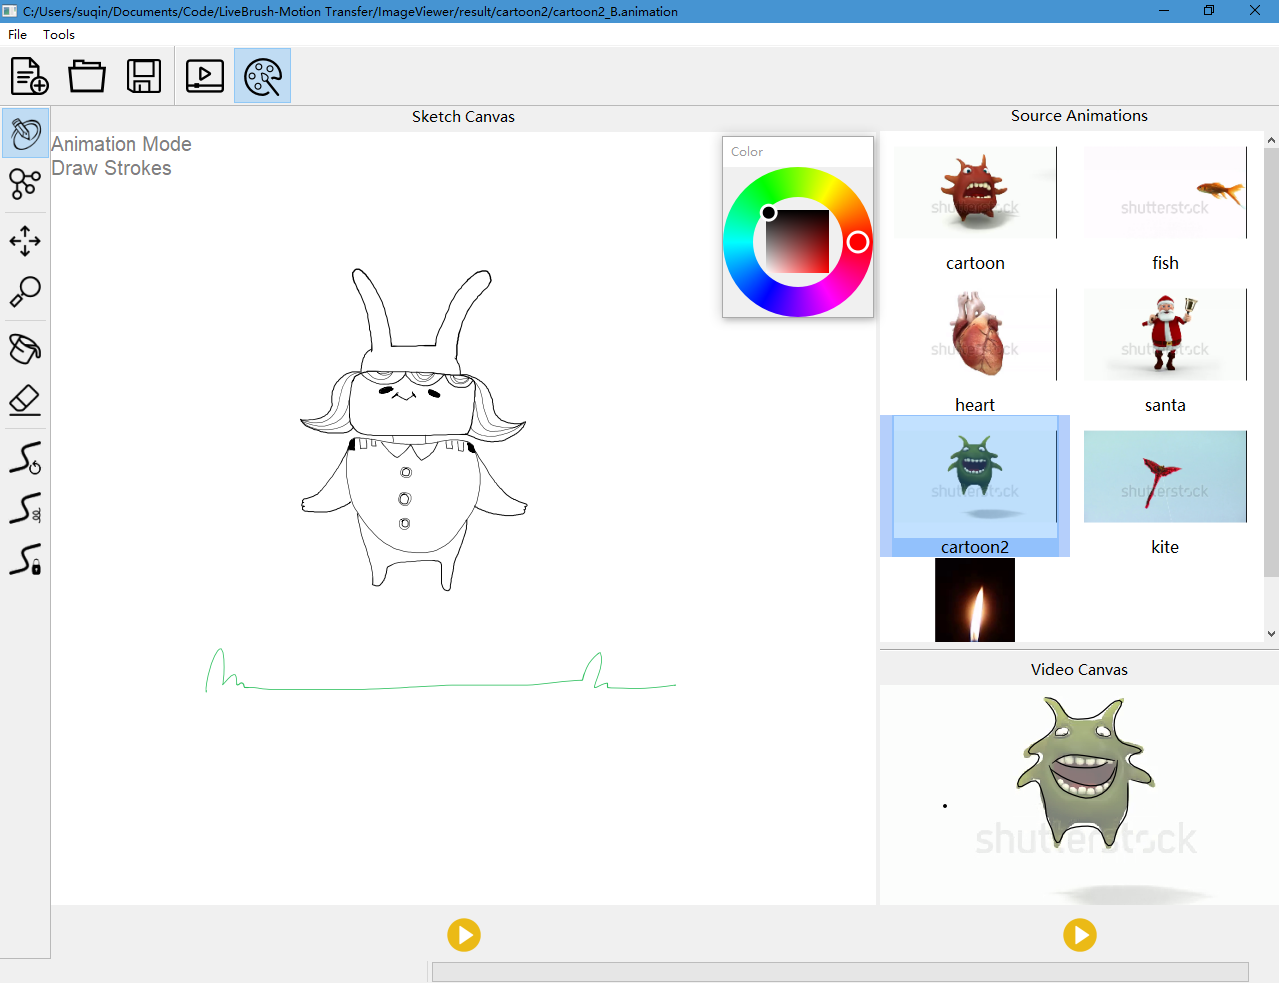
\includegraphics[width=\linewidth]{images/ui}
%	\caption{User interface of our system.}
%	\label{fig:ui}
%\end{figure}

\subsubsection{Motion Extraction}\label{sec:motion_extraction}

After loading a new video into our system, 
the user first roughly specifies the desired object on {one of the video frames (the first frame by default)}, from which motion will be extracted.
The system suggests an object outline by applying automatic GrabCut segmentation~\cite{Rother:2004}, which works well when the background is clean. Otherwise, the user can quickly draw the correct outline using a pen tool. The extracted object shape will later be aligned with the user-provided sketch for motion transfer.

In the next step, the user defines a set of structural control points inside the object, which are automatically tracked through the entire video. The details about control point extraction are described in Sec.~\ref{feature_extraction}, and our tracking method is described in Sec.~\ref{sec:motion_extraction}.  
The trajectories of these control points represent the object motion, and will be applied to the corresponding control points on the sketch for animation. 
Given that tracking is not always perfect, our interface also provides manual tools for fine-tuning the extracted motion by adding, removing or adjusting the control points. The motion trajectories are updated in real time and visualized to the user during the editing process (see Fig.~\ref{fig:ui2}, Left). 
%A screen shot of this interface is shown in Fig.~\ref{fig:user_interface}.
\begin{figure}
	\centering
	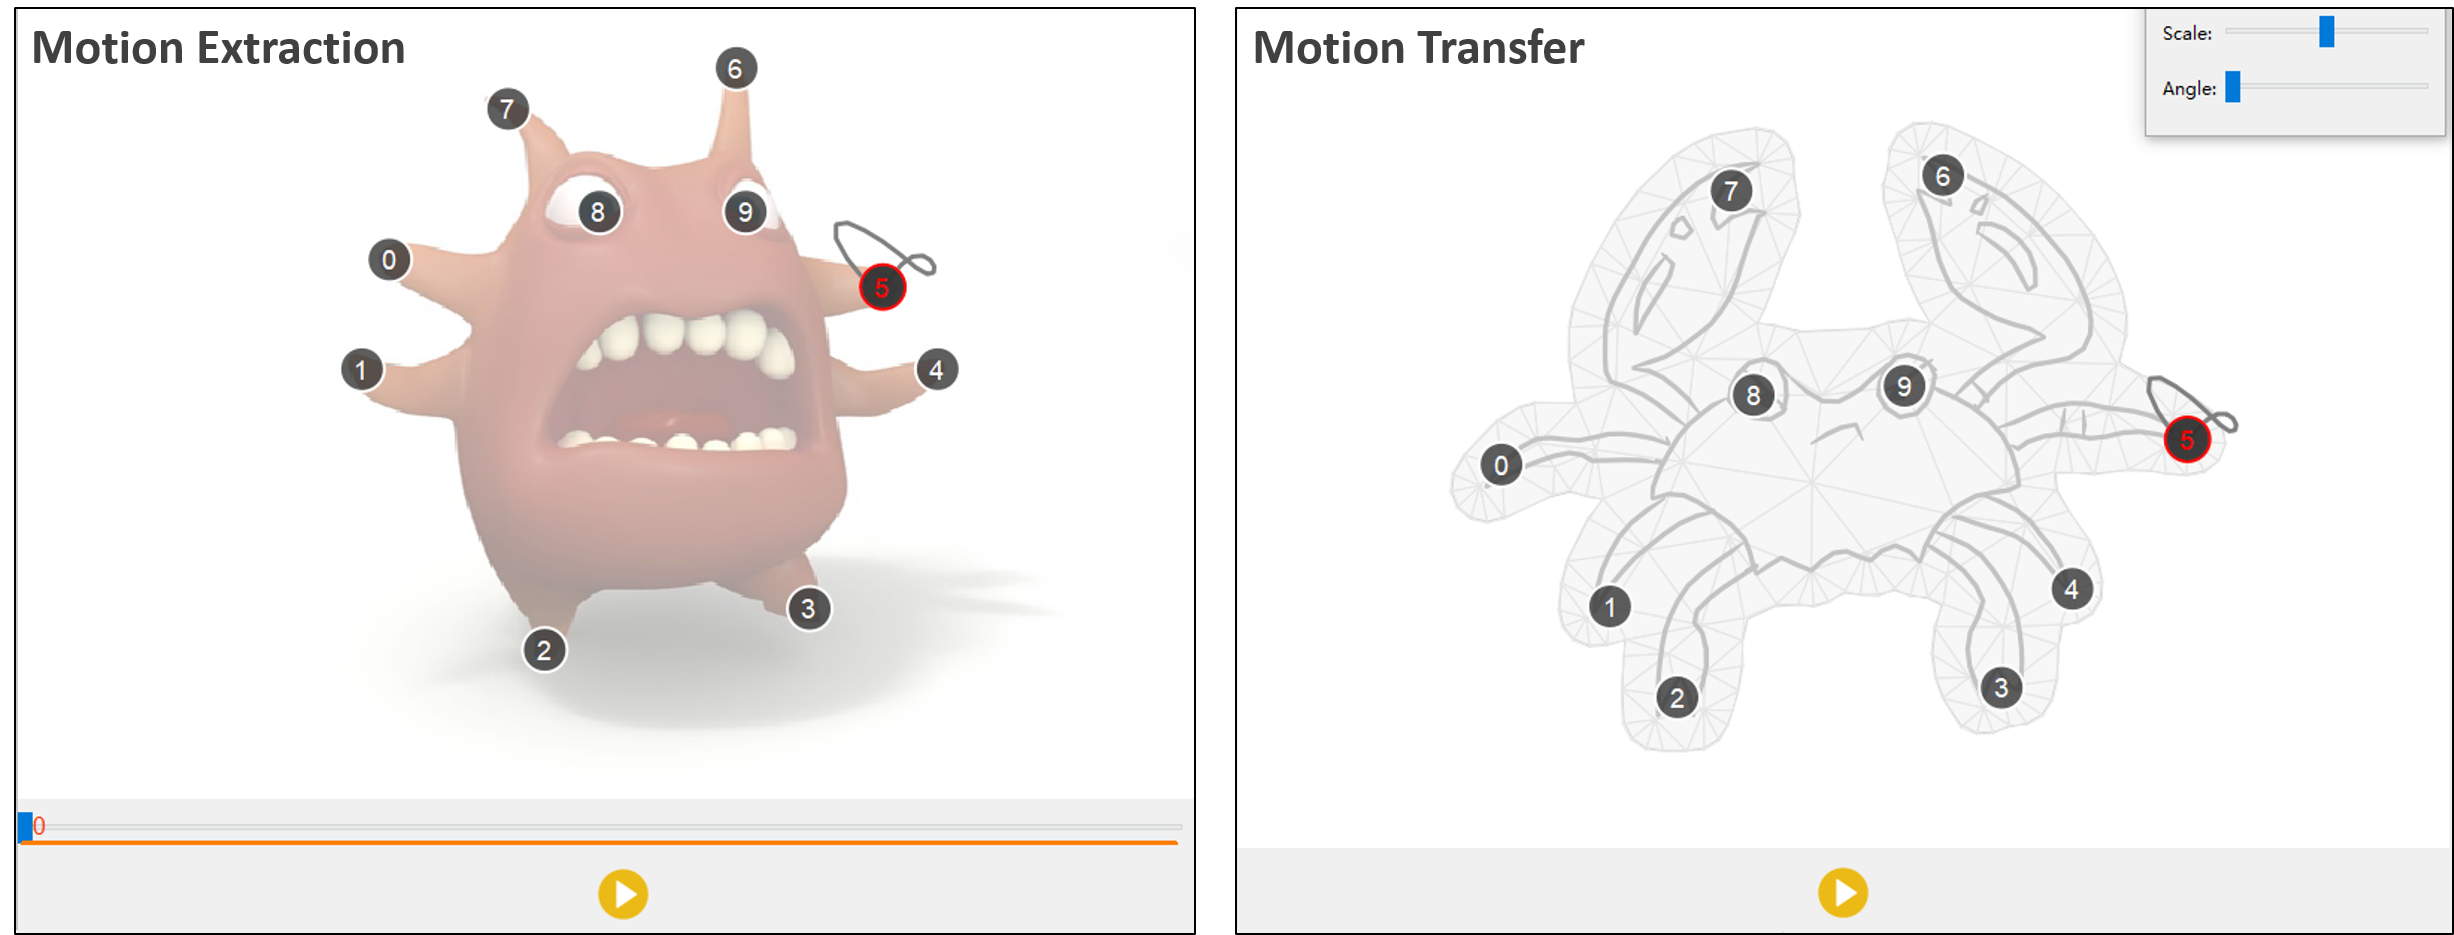
\includegraphics[width=\linewidth]{images/ui2}
	\caption{Our user interfaces. Left: motion extraction UI, where control points are defined and tracked in the input video. Right: motion transfer UI, where the position and motion of the control points are used to drive the sketch. The corresponding control points on the video and sketch are labeled with the same numbers.}
	\label{fig:ui2}
\end{figure}

\begin{figure}
	\centering
	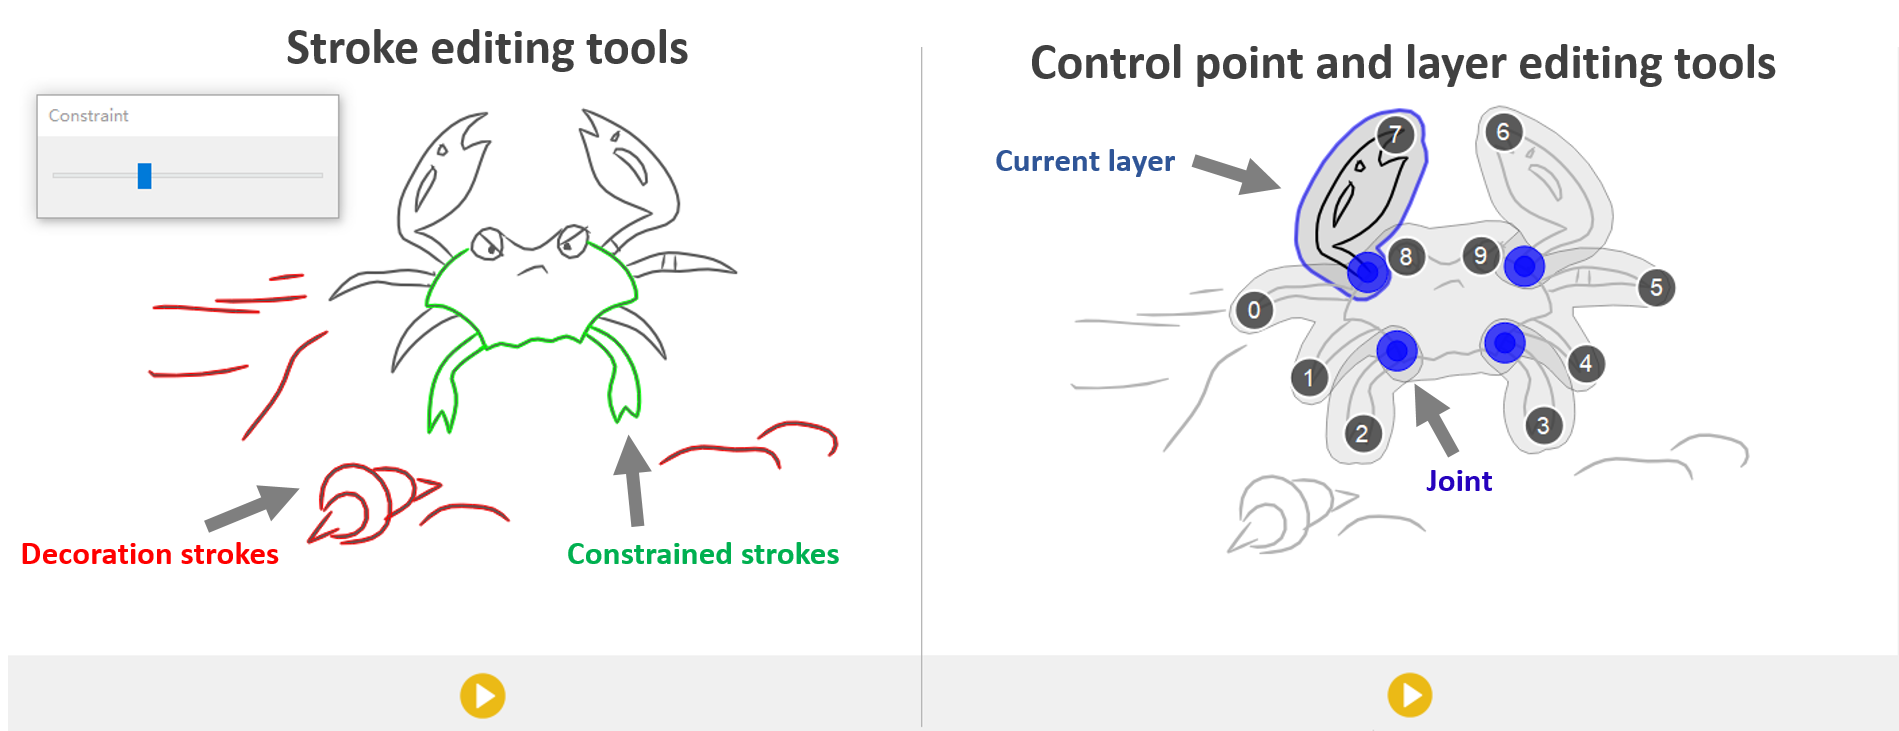
\includegraphics[width=\linewidth]{images/othertools}
	\caption{Interactive tools for motion transfer. Left: the user can label selected strokes as decoration strokes (i.e., no motion), or add strong shape rigidity constraints to strokes. Right: the user can group several strokes as a new layer to animate them independently from other strokes, or add/move automatically initiated joints in the layer intersection regions. }
	\label{fig:othertools}
\end{figure}

\subsubsection{Motion Transfer}
As the target for motion transfer, the user either imports an existing sketch or draws a new one in our system.
The system automatically computes shape correspondence between the video object and the user-provided sketch, in order to map the control point trajectories to the sketch (Sec.~\ref{sec:cp_transfer}). These mapped control points are used as constraints in a mesh deformation process to drive the animation, as detailed in Sec.~\ref{motion_transfer}. The user can immediately review the animation result without any additional manual operation.

Our interface also provides interactive tools for fine-tuning the automatically-generated sketch animation, as shown in Fig.~\ref{fig:othertools}. 
First, it allows the user to adjust the spatial positions of the control points on the sketch, which are automatically inferred from the control points on the video object. 
% User first select one edit the spatial correspondence between sketch and video by two control points 
%First, our system shows a set of control points for user to do the animation editing. User can move the control points to change their influencing regions.
Another useful tool is ``Rigidity Stroke'', which can be used to prevent local shape distortion during the animation.
The user can also use a ``Static Stroke'' to mark sketch components that are to remain stationary, like those for background decoration.

One important feature of our system is its ability to decompose a sketch and animate it in multiple layers (see Fig.~\ref{fig:othertools}, Right). This is particularly useful for handling self-occlusions, which are common for video objects with complex motion. To create such layers, the user can use a ``Layer Brush'' to paint over strokes that should be grouped together, based on the semantics of the object and its motion. We also provide an interface for users to refine the automatically generated joints between layers to fine-tune the animation. Please refer to Sec.~\ref{sec:multi-layer_animation} for more details.
% The user can additionally add or move joints' positions if needed to fine-tune the animation.

